\section{\texorpdfstring{\WZ}{WZ} Background}
\label{sec:bkg_WZ}

This is the primary background in our search (about 51\,\%). To estimate this process, we define the \WZ control region by 3 leptons, an on-\Z OSSF pair, and $50\,\GeV < \MET < 100\,\GeV$. We use \WZ MC with fully leptonic decays and normalize the total number of events in the control region, after subtracting other backgrounds.

We use the $M_\textrm{T}$ distribution (Fig.~\ref{fig:WZ}) to check the \WZ normalization in the control region, where $M_\textrm{T}$ is defined as
$$M_\textrm{T} = \sqrt{2 \MET p_\textrm{T}^\ell \left( 1 - \cos\measuredangle(\vec E_\textrm{T}^\text{miss}, \vec p_\textrm{T}^{\,\ell}) \right)},$$ and $\ell$ refers to the lepton that is not part of the OSSF pair. In case of ambiguity, the OSSF pair is defined as the one whose invariant mass is closer to the \Z boson mass.

\begin{figure}
\begin{center}
	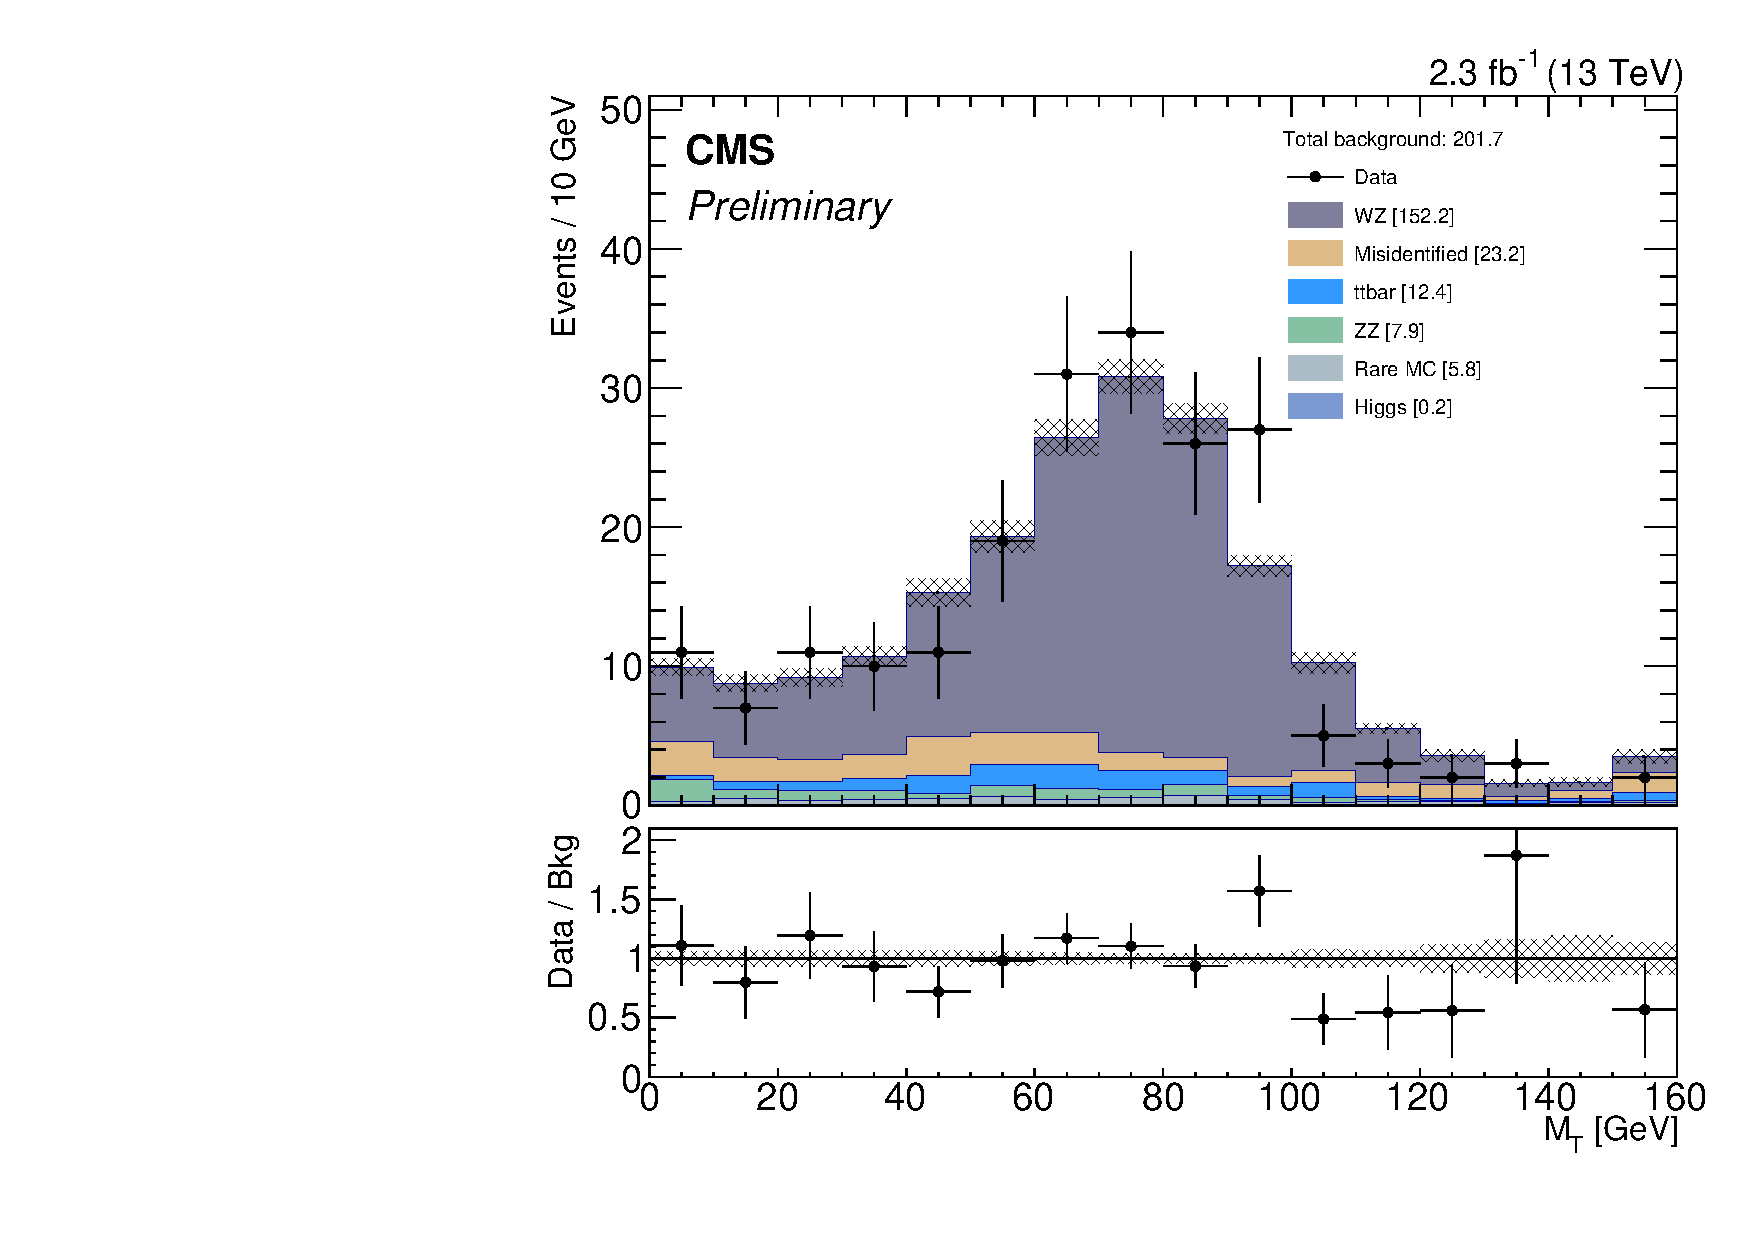
\includegraphics[width=.7\textwidth]{Background/bkg_WZ/WZ_MET50to100_MT}
	\caption{$M_\textrm{T}$ distribution in the \WZ-dominated control region (last bin includes overflow). Uncertainty bands include both statistical and systematic uncertainties, with the exception of the \WZ normalization uncertainty.
	\label{fig:WZ}}
\end{center}
\end{figure}

We validate the prediction in the adjoining $100\,\GeV < \MET < 150\,\GeV$ region and assign a systematic uncertainty of 50\,\% based on the variation of the normalization factor between the normalization region and the validation region.
